%!TEX root = ../../template.tex
\section{DOAS Tomography}%
\label{sec:litrev_doas_tomography}

The main goal of the \gls{sms} that I am going to address was to
determine a good starting point for the system that I was aiming at. How
is the current literary panorama for DOAS tomography? What is the
novelty level of a drone-based spectroscopic system using tomographic
trajectories? Answering these questions was extremely important for the
(at the time) future of this project. They were also the basis for the
definition of the article's research question: \textbf{What is the
current status of DOAS tomography technology?}

Such a broad research question would be impossible to answer from direct
literary research, so I partitioned my approach in three narrower parts.
What does the typical hardware used for DOAS tomography look like? What
kind of software are researchers using for this effect? What are the
most common algorithms in use by the community? These questions are
summarised in Table~\ref{tab:lit_rev_RQ1}.

\begin{table}[htb]
\centering
\small
\caption{Research question slicing}
\label{tab:lit_rev_RQ1}
    \begin{tabularx}{\textwidth}{lX}
        \toprule
        \textbf{Original} & What is the current status of the technology used in
        tomographic DOAS? \\
        \textbf{RQ1} & Is there a typical hardware setup used in tomographic
        DOAS studies? \\
        \textbf{RQ2} & Is there a standard software used to perform these
        analysis? \\
        \textbf{RQ3} & What are the algorithms more commonly used?\\\bottomrule
    \end{tabularx}
\end{table}

Preliminary searches revealed that it would be difficult finding many
sources on tomographic \gls{DOAS}. This was a defining moment on the
article's development, since it meant that both the search terms and the
used libraries would have to be broad, putting more pressure on the
filtering operation.

Preliminary searches, ran as tests for this study, indicated that there
were a very low number of studies in \gls{DOAS} tomography, in
comparison to other subjects to which this methodology is commonly
applied. As consequence, the search terms were purposefully chosen as to
maintain a broad scope and retrieve the largest possible amount of
articles. The selected terms were: \textbf{DOAS atmospher*
tomography}\footnote{The asterisk acts as a wildcard.}. The same
strategy was applied to the selection of electronic libraries, as these
preliminary searches revealed that there was a poor availability of
relevant information in the most commonly used libraries. This in itself
motivated a two stage approach to the search effort, in which we use
several libraries to complement an initial \gls{gs} search. Libraries
used are summarised in Table~\ref{tab:lit_rev_libraries}. Determining
how a paper was to be used in my paper was a matter of applying the
inclusion and exclusion filters presented in
Table~\ref{tab:lit_rev_filters}, according to a particular algorithm
that is presented in its flowchart form in
Figure~\ref{fig:lit_rev_search_flowchart}. 

Inclusion is a binary function. Either a paper is included or it is not.
How then, should a paper be ranked once it is included? This is tackled
by defining an objective metric with which to measure the paper's
influence in the field. There are many ways to do this, but I have
chosen to apply the formula in
Equation~\ref{eq:lit_rev_paper_quality_metric}. This formula uses the
paper's journal ranking, the number of citations it has garnered and its
age to determine how much it is relevant to the investigation I was
conducting.

\begin{table}[htb]
\centering
\caption{Electronic libraries used in the \gls{sms} study.}
\label{tab:lit_rev_libraries}
\begin{tabularx}{\textwidth}{ll}
\toprule
\textbf{Library}          & \textbf{URL}\\
\midrule
\gls{gs}   & https://scholar.google.com/\\
\gls{wok}& https://webofknowledge.com\\
\gls{sd}   & https://www.sciencedirect.com\\
\bottomrule
\end{tabularx}
\end{table}

\begin{table}[htb]
\centering
\caption{Selection filters in use for this study's search.}
\label{tab:lit_rev_filters}
\begin{tabularx}{\textwidth}{lXl}%{@{}cll@{}}
\toprule
\multicolumn{1}{l}{} & \textbf{Criterium} & \textbf{Definition} \\ \midrule
\multirow{1}{*}{\textbf{Exc. Criteria}} & EC1 & Satellite data papers
are not accepted \\
\midrule
\multicolumn{1}{l}{\multirow{3}{*}{\textbf{Inc. Criteria}}} & IC1 &
Results must be journal papers \\
\multicolumn{1}{l}{} & IC2 & Results must be about Tomographic DOAS \\ 
\multicolumn{1}{l}{} & IC3 & Results must be written in English \\ 
\bottomrule
\end{tabularx}
\end{table}

\begin{equation}
    \centering
    \label{eq:lit_rev_paper_quality_metric}
    S = Q_{i} \cdot \frac{C_{i}}{Age_{i}}
\end{equation}

\begin{figure}[htpb]
    \centering
    \includegraphics[width=\linewidth]{img/pdf/asd_flowchart.pdf}
    \caption{Conduction stage flowchart. Libraries are searched
    independently through \emph{Publish or Perish}~\cite{Harzing}, but
    results must be checked to ensure they are not counted twice, due to the
    imbalance of power between \gls{gs}'s search engine and the others.}
    \label{fig:lit_rev_search_flowchart}
\end{figure}

The application of the aforementioned methods has rendered what is
summarised in two tables. Table~\ref{tab:lit_rev_high_level_results}
presents a high-level representation of the search results.
Table~\ref{tab:lit_rev_selected_articles} presents all selected papers,
as well as their score according to the formula of
Equation~\ref{eq:lit_rev_paper_quality_metric}. The following subsection
includes my observations on the hypothesis explored through the selected
papers and how I can use this in my research.

\begin{table}[htb]
\centering
\caption{Search results summary.}
\label{tab:lit_rev_high_level_results}
\begin{tabular}{@{}lccccr@{}}
\toprule
\textbf{Library} & \textbf{Results} & \textbf{Excluded} & \textbf{In \gls{gs}} & \textbf{Final} & \textbf{Weight in study} \\ \midrule
\textbf{\gls{gs}} & 37 & 25 & 0 & 12 & 92,31\% \\
\textbf{Scopus} & 15 & 3 & 12 & 0 & 0\% \\
\textbf{WoS} & 9 & 1 & 7 & 1 & 7,69\% \\
\midrule
\textbf{Total}& \textbf{61} & \textbf{29} & \textbf{19} &\textbf{13} & \textbf{100,00\%} \\ \bottomrule
\end{tabular}
\end{table}


\begin{table}[htb]
    \centering
    \small
    \caption{References and relevant data for the selected papers,
        including their score, which was calculated according to
        Equation~\ref{eq:lit_rev_paper_quality_metric}.}
    \label{tab:lit_rev_selected_articles}
    \begin{tabular}{@{}llllll@{}}
    \toprule
    \textbf{Number} & \textbf{Reference} & \textbf{Quartile} &
    \textbf{Citations} & \textbf{Year} & \textbf{Score} \\ \midrule
    \textbf{1} & \cite{Hartl2006} & 1 & 35 & 2006 & 2,69 \\
    \midrule
    \textbf{2} & \cite{Hartl2005} & 1 & 2 & 2005 & 0,14 \\
    \midrule
    \textbf{3} & \cite{Laepple2004} & 1 & 30 & 2004 & 2,00 \\
    \midrule
    \textbf{4} & \cite{Pundt2005} & 2 & 1 & 2005 & 0,05 \\
    \midrule
    \textbf{5} & \cite{Murphy2003} & 3 & 6 & 2003 & 0,19 \\
    \midrule
    \textbf{6} & \cite{Frins2006} & 1 & 8 & 2006 & 0,62 \\
    \midrule
    \textbf{7} & \cite{Johansson2009} & 2 & 26 & 2009 & 1,95 \\
    \midrule
    \textbf{8} & \cite{ODriscoll2003} & 4 & 0 & 2003 & 0,00 \\
    \midrule
    \textbf{9} & \cite{Pundt2006} & 1 & 12 & 2006 & 0,92 \\
    \midrule
    \textbf{10} & \cite{Pundt2005b} & 1 & 42 & 2005 & 3,00 \\
    \midrule
    \textbf{11} & \cite{ODriscoll2003a} & 4 & 1 & 2003 & 0,02 \\
    \midrule
    \textbf{12} & \cite{Mettendorf2006} & 1 & 4 & 2006 & 0,31 \\
    \midrule
    \textbf{13} & \cite{Casaballe2017} & 1 & 2 & 2017 & 1,00 \\ \bottomrule
    \end{tabular}
\end{table}



\subsection{Paper Analysis - The DOAS Tomography State of the Art}%
\label{sub:paper_analysis_the_doas_tomography_state_of_the_art}

The first identifiable pattern is the marked prevalence of active
\gls{DOAS} systems. 11 out of the 13 retrieved papers describe or
consider an active \gls{DOAS} system of some kind. As stated in
Section~\ref{sec:doas}, active \gls{DOAS} systems do have better
analytical capabilities than their passive counterparts, although that
comes at the cost of increased instrument complexity and operational
costs. 

Another immediate conclusion is that there is a "dominant" study. Almost
half of the papers found originated from the BABII campaign, in which a
group of researchers set out to quantify pollution through \gls{DOAS}
tomography along a busy German motorway, in the beginning of the
21\textsuperscript{st} century~\cite{Hartl2005, Hartl2006,
Laepple2004, Pundt2005, Pundt2006, Pundt2005a, Mettendorf2005}.

All of the active \gls{DOAS} systems were purposely built for their
corresponding experiment (or group of experiments). BABII researchers
used two telescopes with around 200mm diameter and 1m focal length to
simultaneously illuminate 8 retroreflectors that were assembled onto two
towers located on each side of the road. In one of the papers associated
with this initiative, the same telescope instrumentation was used to
validate the 2D reconstruction technique that was going to be used in
the other papers. The campaign's main assembly is illustrated in
Figure~\ref{fig:babii}.

\begin{figure}[htpb]
    \centering
    \includegraphics[width=0.6\linewidth]{img/png/babii_geometry.png}
    \caption{BABII assembly geometry. In this experiment campaign, the
    telescopes illuminated retroreflecting targets that were positioned
    in two steel towers on both sides of a busy motorway in Germany,
    connecting Heidelberg to Mannheim~\cite{Pundt2005a}.}
    \label{fig:babii}
\end{figure}


Another important initiative with respect to \gls{DOAS} tomography was
the study conducted in 2016 by Stutz et al~\cite{Stutz2016}. The
approach in this case was to use a similar telescope to detect the light
emitted by a narrow interval UV LED light source (290nm) to create a
fence line monitoring system for Benzenes, Toluene and Xylene. The team
managed to apply this system in a successful manner in refineries in Los
Angeles and Houston. One of the most interesting aspects of this study
is that it details a tomographic system that could easily be
commercially deployed.

Another type of \gls{DOAS} tomography system was proposed by researchers
in the Cork Institute of Technology~\cite{ODriscoll2003,ODriscoll2003a,
Murphy2003}.  In their three papers, the authors describe \textbf{1)} a
new multipath instrument that significantly increases the amount of
projection information in this kind of application; \textbf{2)} a
tomographic reconstruction algorithm based on evolutionary algorithms;
and \textbf{3)} the application of \gls{DOAS} tomography to a simulated
urban canyon scenario. Although all three papers present technological
innovation, it would not be fair not to say that from a strictly
literary point of view, these were among the weakest retrieved by the
search process.

Regarding passive DOAS applications, the two papers we have found come
with two completely different paradigms. The first
article~\cite{Johansson2009} was written in 2009 and details the
application of a tomographic inversion algorithm to a scanning DOAS
application, designed to work with trace gas plumes like the ones above
volcanoes or power stations. The team present a system composed of two
DOAS devices, with sufficient distance with themselves as to allow
tomographic reconstruction, but sufficiently small to allow the light
path to be considered a straight line from the point of last scattering
to the detector. The authors applied an adapted version of the Lower
Third Derivative (LTD) algorithm to the projections obtained by pointing
the set of fixed DOAS apparatus towards the plume in different angles.
Besides simulations for their proposed method, the authors have also
conducted practical experiments, both over a power plant in Spain and a
volcano in Italy. Results from these experiments display a good
agreement between reality and simulation results, proving the
technique's validity.

The second Passive DOAS application is a paper published by Frins et
al.~\cite{Frins2006}. In this study, the researchers detail a particular
application in which they measure light coming from bright and
nonreflecting sun-illuminated objects in their field of view. They use
this light to retrieve column density values for a number of trace
gases. The proposed method also includes a way with which to remove the
stratospheric contribution that appears in the measured light besides
the target column. The authors discuss how radiative transfer can
influence measurements, but they also present a number of approaches to
mitigate this problem, ensuring the validity of their approach.  Besides
presenting the method, the authors also describe an experiment they
conducted by assembling and manoeuvring a DOAS system on top of a
building in Heidelberg, Germany.

\begin{figure}[htpb]
    \centering
    %left bottom right top
    \begin{subfigure}[b]{.475\textwidth}
        \centering
        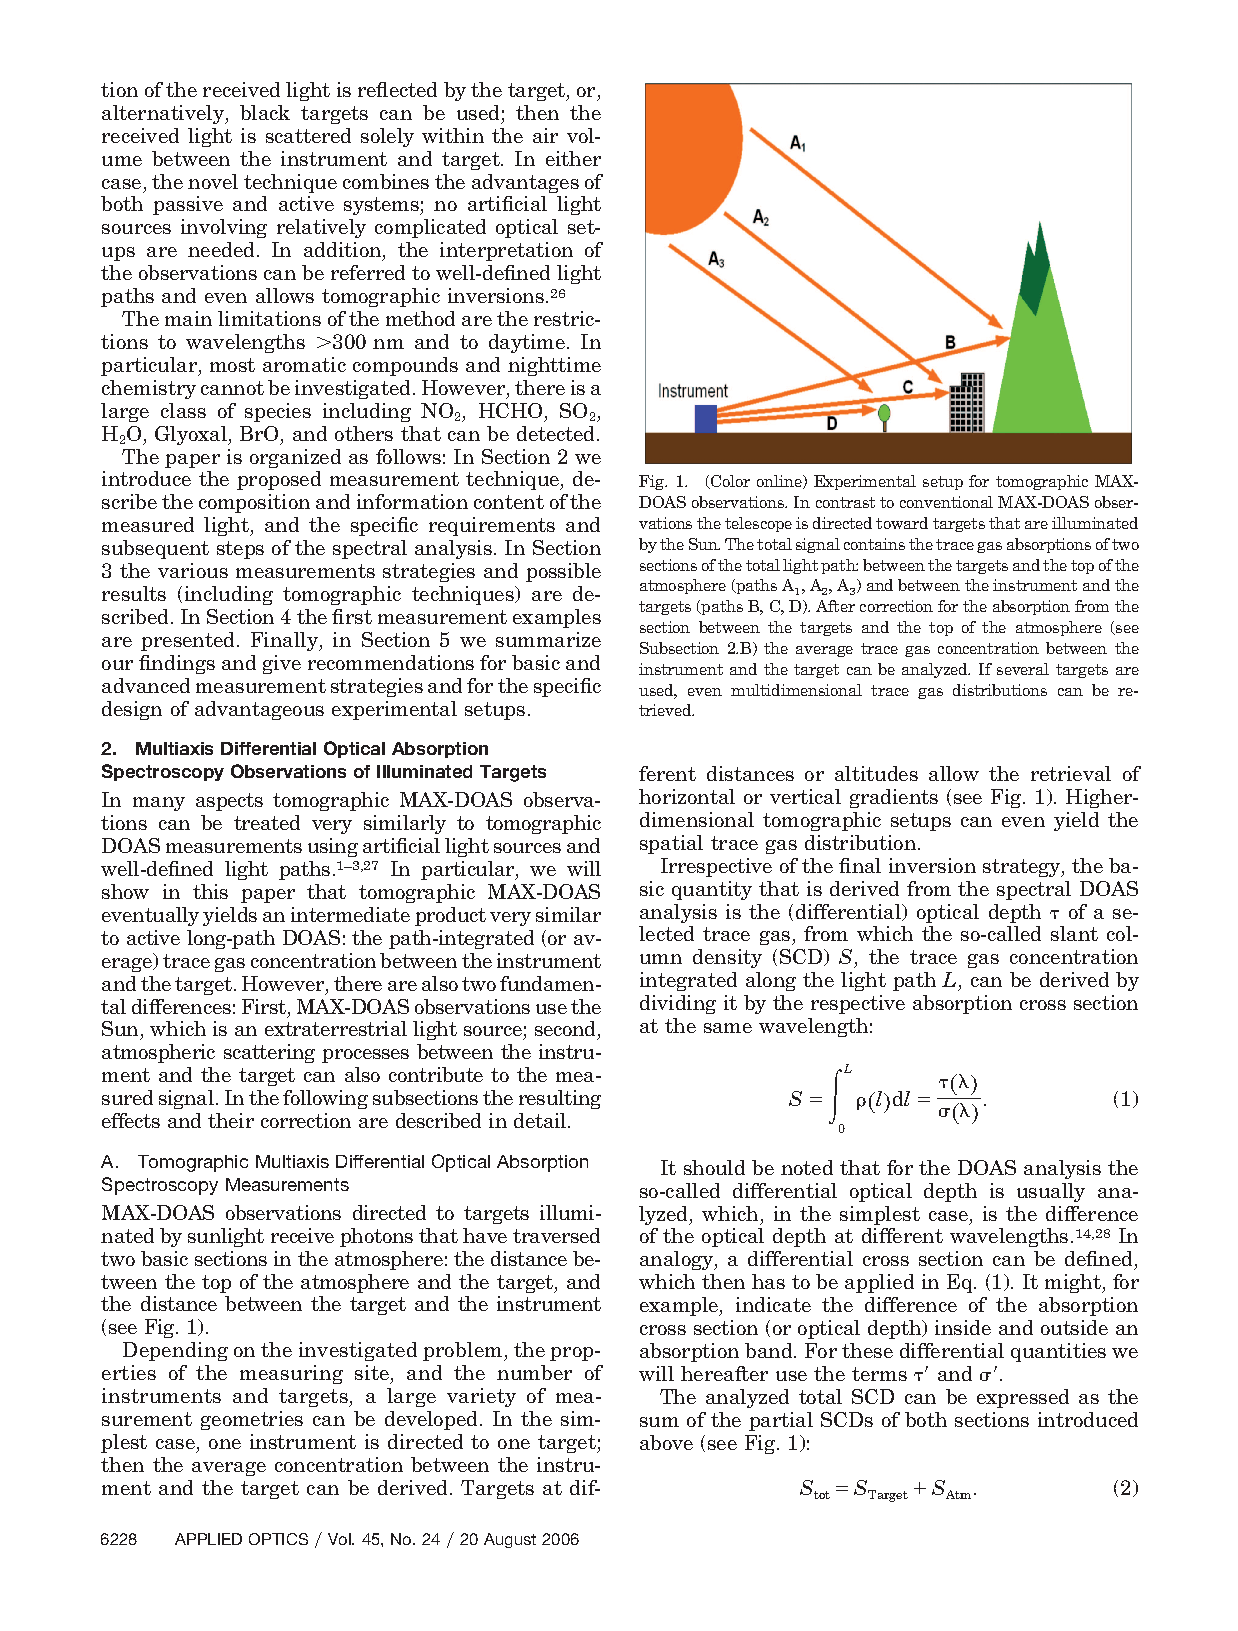
\includegraphics[trim=10.8cm 19.7cm 2cm 2cm, clip, %...
        width=\textwidth]{img/pdf/frinsSchematics_p2.pdf}
        \caption{Schematic representation of Frins's
        assembly~\cite{Frins2006}.}
        \label{fig:frins_schem_1}
    \end{subfigure}
    \hfill
    \begin{subfigure}[b]{.475\textwidth}
        \centering
        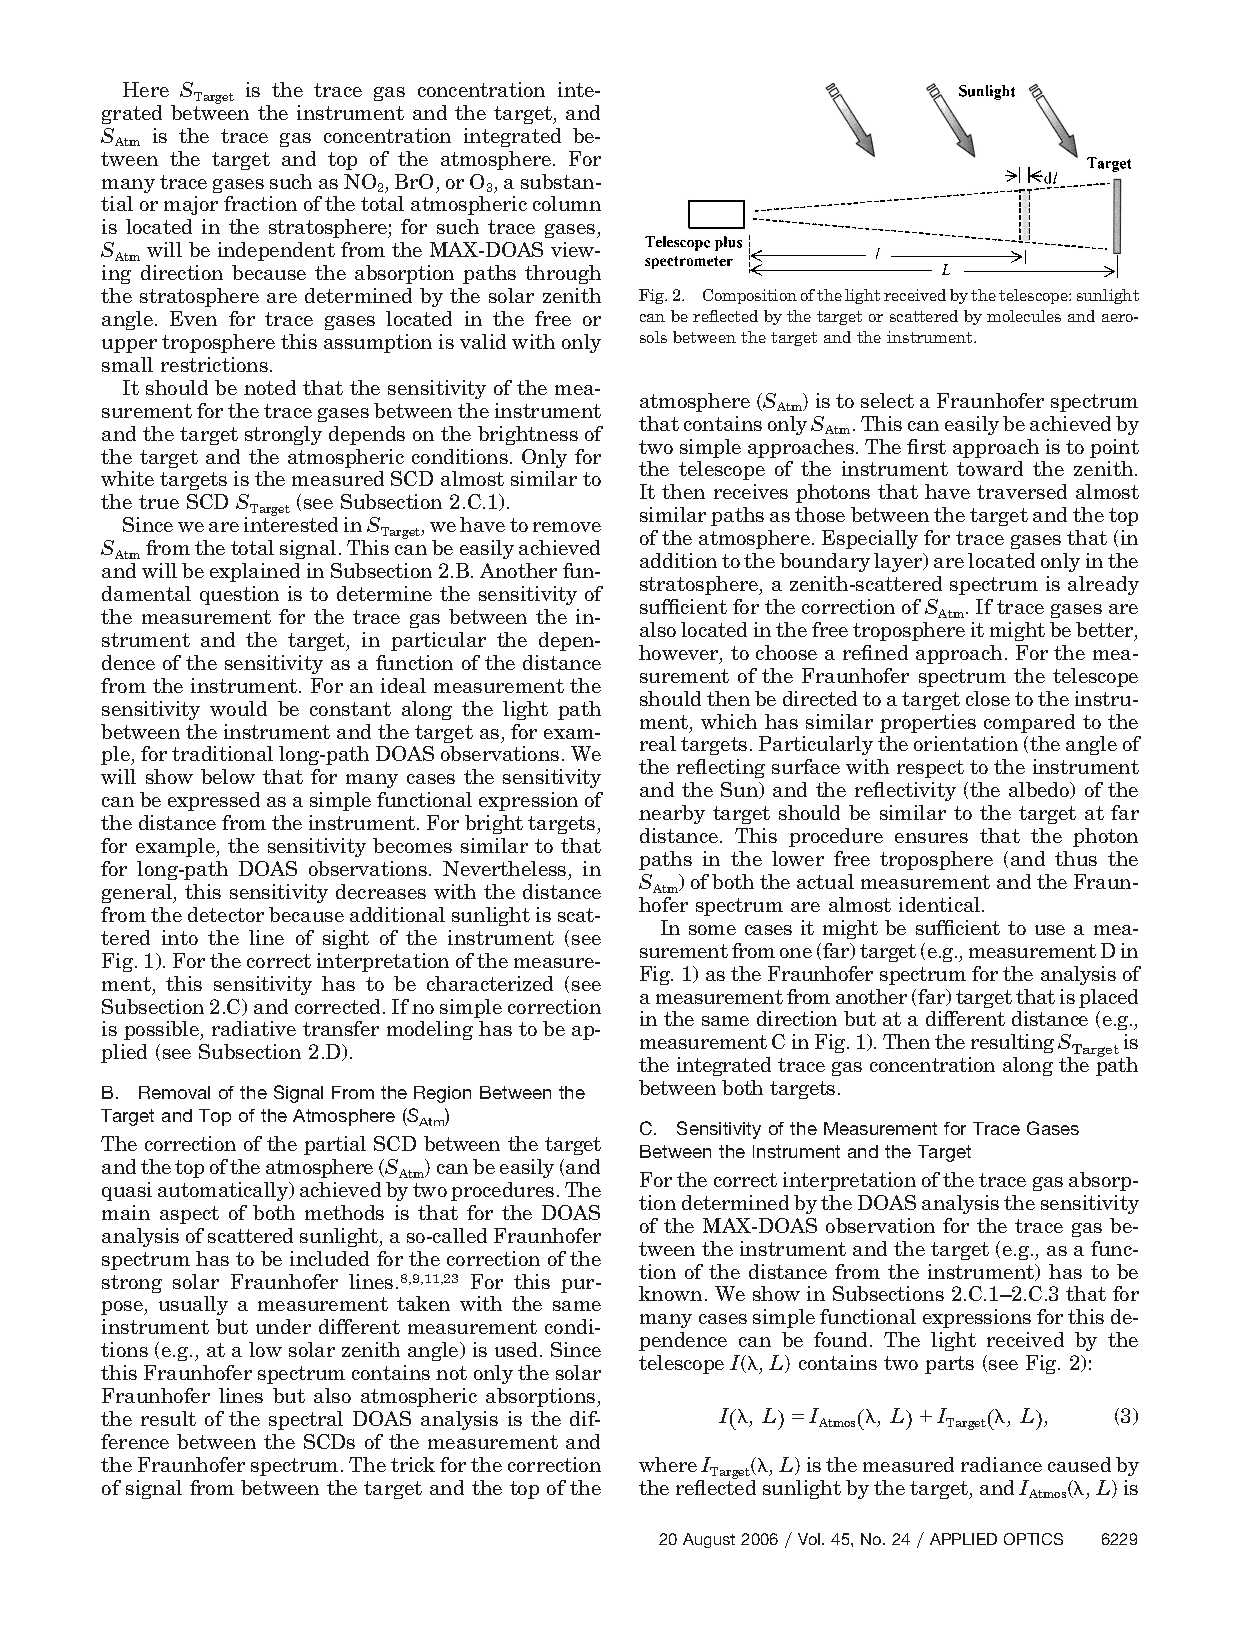
\includegraphics[trim=10.8cm 22.8cm 1cm 1cm, clip, %...
        width=\textwidth]{img/pdf/frinsSchematics_p3.pdf}
        \caption{The physical principle behind Frins's
        paper~\cite{Frins2006}.}
        \label{fig:frins_schem_2}
    \end{subfigure}
    \caption{Erna Frins's paper~\cite{Frins2006} proposes a very
        relevant passive \gls{DOAS} application that can conceptually be
        employed in a \gls{DOAS} tomography scenario. In this 2006
        paper, the authors use multi-axis measurements of
        sun-illuminated targets to estimate absorption paths without
        using radiative transfer models.}
    \label{fig:ernafrins}
\end{figure}

In summary, the search has found that active tomographic \gls{DOAS} is
far more common than the passive counterpart (11 out of 13 articles
discussed this method). This preference can be explained by the fact
that the results produced by this kind of system are generally superior
to those obtained by passive methods. However, passive applications are
normally much less demanding on a technical level, and are simpler to
run and assemble.  Much as a result of this, we have also identified
that the systems used in the literature were not mobile or had a very
low mobility level which in turn caused that all the systems were
working with low projection numbers. This should be taken into account
in future research on the topic. As a final note, we would also like to
point out that there is no commercially available systems for this kind
of application, although some of the articles, like the one by Stutz in
2016~\cite{Stutz2016} detail systems which could easily be adapted to
that end.

